% Options for packages loaded elsewhere
\PassOptionsToPackage{unicode}{hyperref}
\PassOptionsToPackage{hyphens}{url}
\PassOptionsToPackage{dvipsnames,svgnames,x11names}{xcolor}
\documentclass[
  english,
  spanish,
  10pt,
  letterpaper,
]{article}
\usepackage{xcolor}
\usepackage[top=2.3cm,bottom=2.1cm,left=2.2cm,right=2.2cm,headsep=0.5cm]{geometry}
\usepackage{amsmath,amssymb}
\setcounter{secnumdepth}{5}
\usepackage{iftex}
\ifPDFTeX
  \usepackage[T1]{fontenc}
  \usepackage[utf8]{inputenc}
  \usepackage{textcomp} % provide euro and other symbols
\else % if luatex or xetex
  \usepackage{unicode-math} % this also loads fontspec
  \defaultfontfeatures{Scale=MatchLowercase}
  \defaultfontfeatures[\rmfamily]{Ligatures=TeX,Scale=1}
\fi
\usepackage{lmodern}
\ifPDFTeX\else
  % xetex/luatex font selection
\fi
% Use upquote if available, for straight quotes in verbatim environments
\IfFileExists{upquote.sty}{\usepackage{upquote}}{}
\IfFileExists{microtype.sty}{% use microtype if available
  \usepackage[]{microtype}
  \UseMicrotypeSet[protrusion]{basicmath} % disable protrusion for tt fonts
}{}
\usepackage{setspace}
\makeatletter
\@ifundefined{KOMAClassName}{% if non-KOMA class
  \IfFileExists{parskip.sty}{%
    \usepackage{parskip}
  }{% else
    \setlength{\parindent}{0pt}
    \setlength{\parskip}{6pt plus 2pt minus 1pt}}
}{% if KOMA class
  \KOMAoptions{parskip=half}}
\makeatother
\usepackage{longtable,booktabs,array}
\usepackage{caption}
\captionsetup[table]{skip=6pt}
\newcounter{none} % for unnumbered tables
\usepackage{calc} % for calculating minipage widths
% Correct order of tables after \paragraph or \subparagraph
\usepackage{etoolbox}
\makeatletter
\patchcmd\longtable{\par}{\if@noskipsec\mbox{}\fi\par}{}{}
\makeatother
\usepackage{graphicx}
\makeatletter
\newsavebox\pandoc@box
\newcommand*\pandocbounded[1]{% scales image to fit in text height/width
  \sbox\pandoc@box{#1}%
  \Gscale@div\@tempa{\textheight}{\dimexpr\ht\pandoc@box+\dp\pandoc@box\relax}%
  \Gscale@div\@tempb{\linewidth}{\wd\pandoc@box}%
  \ifdim\@tempb\p@<\@tempa\p@\let\@tempa\@tempb\fi% select the smaller of both
  \ifdim\@tempa\p@<\p@\scalebox{\@tempa}{\usebox\pandoc@box}%
  \else\usebox{\pandoc@box}%
  \fi%
}
% Set default figure placement to htbp
\def\fps@figure{htbp}
\makeatother
% definitions for citeproc citations
\NewDocumentCommand\citeproctext{}{}
\NewDocumentCommand\citeproc{mm}{%
  \begingroup\def\citeproctext{#2}\cite{#1}\endgroup}
\makeatletter
 % allow citations to break across lines
 \let\@cite@ofmt\@firstofone
 % avoid brackets around text for \cite:
 \def\@biblabel#1{}
 \def\@cite#1#2{{#1\if@tempswa , #2\fi}}
\makeatother
\newlength{\cslhangindent}
\setlength{\cslhangindent}{1.5em}
\newlength{\csllabelwidth}
\setlength{\csllabelwidth}{3em}
\newenvironment{CSLReferences}[2] % #1 hanging-indent, #2 entry-spacing
 {\begin{list}{}{%
  \setlength{\itemindent}{0pt}
  \setlength{\leftmargin}{0pt}
  \setlength{\parsep}{0pt}
  % turn on hanging indent if param 1 is 1
  \ifodd #1
   \setlength{\leftmargin}{\cslhangindent}
   \setlength{\itemindent}{-1\cslhangindent}
  \fi
  % set entry spacing
  \setlength{\itemsep}{#2\baselineskip}}}
 {\end{list}}
\usepackage{calc}
\newcommand{\CSLBlock}[1]{\hfill\break\parbox[t]{\linewidth}{\strut\ignorespaces#1\strut}}
\newcommand{\CSLLeftMargin}[1]{\parbox[t]{\csllabelwidth}{\strut#1\strut}}
\newcommand{\CSLRightInline}[1]{\parbox[t]{\linewidth - \csllabelwidth}{\strut#1\strut}}
\newcommand{\CSLIndent}[1]{\hspace{\cslhangindent}#1}
\ifLuaTeX
\usepackage[bidi=basic,shorthands=off,es-noshorthands,es-nodecimaldot]{babel}
\else
\usepackage[bidi=default,shorthands=off,es-noshorthands,es-nodecimaldot]{babel}
\fi
\ifLuaTeX
  \usepackage{selnolig} % disable illegal ligatures
\fi
\setlength{\emergencystretch}{3em} % prevent overfull lines
\providecommand{\tightlist}{%
  \setlength{\itemsep}{0pt}\setlength{\parskip}{0pt}}
% Estilo Diablos Rojos para el documento técnico: rojo + negro, Libertinus para el texto, Fira Sans para la estructura.
% Se incluye con pandoc -H diablos.tex (ver build.sh). Solo usa paquetes y fuentes de TeX Live: compila igual en cualquier máquina.
\usepackage{libertinus}
\usepackage[scale=0.92,lining,tabular]{FiraSans}
\renewcommand{\familydefault}{\rmdefault}
\usepackage{microtype}
\usepackage{xcolor}
\definecolor{diablos}{HTML}{C8102E}
\definecolor{tinta}{HTML}{111111}
\definecolor{gris}{HTML}{5C5C5C}
\definecolor{linea}{HTML}{D9D9D9}
\definecolor{fondo}{HTML}{F6F6F6}
\color{tinta}

% Títulos de sección: número rojo, texto negro, filete fino debajo.
\usepackage{titlesec}
\titleformat{\section}{\sffamily\bfseries\Large\color{tinta}}{\textcolor{diablos}{\thesection}}{0.6em}{}[\vspace{2pt}{\color{linea}\titlerule[0.6pt]}]
\titleformat{\subsection}{\sffamily\bfseries\large\color{tinta}}{\textcolor{diablos}{\thesubsection}}{0.6em}{}
\titlespacing*{\section}{0pt}{16pt plus 3pt minus 2pt}{7pt}
\titlespacing*{\subsection}{0pt}{11pt plus 2pt minus 2pt}{4pt}

% Párrafos y listas compactos.
\setlength{\parskip}{3pt plus 1pt}
\usepackage{enumitem}
\setlist{itemsep=2pt, topsep=3pt, parsep=1pt, leftmargin=1.4em}
\setlist[itemize]{label=\textcolor{diablos}{\rule[0.25ex]{0.45em}{0.45em}}}
\setlist[enumerate]{label=\textcolor{diablos}{\sffamily\bfseries\arabic*}, leftmargin=1.6em}

% Tablas en Fira Sans pequeña, filetes booktabs en gris y leyenda con etiqueta roja.
\usepackage{etoolbox}
\usepackage{needspace}
\pretocmd{\section}{\needspace{8\baselineskip}}{}{}
\pretocmd{\subsection}{\needspace{5\baselineskip}}{}{}
\AtBeginEnvironment{longtable}{\sffamily\small\renewcommand{\arraystretch}{1.18}}
\usepackage{colortbl}
\arrayrulecolor{tinta}
\usepackage{caption}
\captionsetup{font={small,sf}, labelfont={bf,color=diablos}, labelsep=period, justification=raggedright,
  singlelinecheck=false, skip=5pt}
\captionsetup[figure]{justification=centering, singlelinecheck=true}

% Encabezado y pie.
\usepackage{fancyhdr}
\pagestyle{fancy}
\fancyhf{}
\fancyhead[L]{\sffamily\footnotesize\textcolor{diablos}{\textbf{Stuff+ 2240}}\hspace{0.6em}\textcolor{gris}{Documento técnico v2}}
\fancyhead[R]{\sffamily\footnotesize\textcolor{gris}{ISAC Sports Analytics Hackathon 2026 · Diablos Rojos}}
\fancyfoot[R]{\sffamily\footnotesize\textcolor{tinta}{\textbf{\thepage}}}
\renewcommand{\headrulewidth}{0.8pt}
\renewcommand{\headrule}{\hbox to\headwidth{\color{diablos}\leaders\hrule height \headrulewidth\hfill}}
\fancypagestyle{plain}{\fancyhf{}\renewcommand{\headrulewidth}{0pt}\renewcommand{\headrule}{}%
  \fancyfoot[R]{\sffamily\footnotesize\textbf{\thepage}}}

% Rutas de reports/ (código en línea) en gris y más pequeñas: son trazabilidad, no texto.
\let\diablosTT\texttt
\renewcommand{\texttt}[1]{{\color{gris}\fontsize{8.2}{10}\selectfont\diablosTT{#1}}}
% Bibliografía compacta.
\AtBeginEnvironment{CSLReferences}{\small\setlength{\parskip}{1pt}}

% Portada en la primera página: franja roja, título en Fira Sans y metadatos.
\makeatletter
\renewcommand{\maketitle}{%
  \thispagestyle{plain}%
  \noindent{\color{diablos}\rule{\linewidth}{5pt}}\par\vspace{10pt}%
  \noindent{\sffamily\footnotesize\bfseries\color{diablos}\MakeUppercase{Documento técnico v2}}\par
  \vspace{6pt}%
  \noindent{\sffamily\bfseries\fontsize{21}{25}\selectfont\color{tinta}\@title}\par
  \vspace{6pt}%
  \noindent{\sffamily\large\color{gris}Equipo Diablos Rojos · ISAC Sports Analytics Hackathon 2026}\par
  \vspace{8pt}%
  \noindent{\sffamily\small\color{tinta}\@author\hspace{0.8em}\textcolor{linea}{|}\hspace{0.8em}\@date}\par
  \vspace{4pt}{\color{tinta}\rule{\linewidth}{1.4pt}}\par\vspace{6pt}}
\makeatother

\addto\captionsspanish{\renewcommand{\tablename}{Tabla}\renewcommand{\figurename}{Figura}}
\usepackage{bookmark}
\IfFileExists{xurl.sty}{\usepackage{xurl}}{} % add URL line breaks if available
\urlstyle{same}
% fallback for those not using the hyperref driver hyperxmp:
\makeatletter
\@ifundefined{xmpquote}{\newcommand{\xmpquote}[1]{#1}}{}
\makeatother
\hypersetup{
  pdftitle={Stuff+ 2240: calidad de pitcheo ajustada por la densidad del aire del Harp Helú},
  pdfauthor={Equipo Stuff+ 2240},
  pdflang={es},
  colorlinks=true,
  linkcolor={diablos},
  filecolor={Maroon},
  citecolor={tinta},
  urlcolor={diablos},
  pdfcreator={LaTeX via pandoc}}

\title{Stuff+ 2240: calidad de pitcheo ajustada por la densidad del aire
del Harp Helú}
\author{Equipo Stuff+ 2240}
\date{Octubre 2026}

\begin{document}
\maketitle

\setstretch{1.06}
\section{Introducción}\label{introducciuxf3n}

El Harp Helú (Ciudad de México, 2,240 m) tiene un aire más ligero que el
de cualquier parque de nivel del mar. Los modelos públicos de calidad de
pitcheo (Stuff+ de FanGraphs, PitchingBot, el Stuff+ de Driveline,
StuffPro de Baseball Prospectus) se entrenan con datos de MLB y su
descripción pública no ajusta por el aire del parque. Para un cuerpo
técnico que evalúa lanzadores en la LMB, el mismo lanzamiento no vale lo
mismo en dos aires distintos.

\textbf{Pregunta del reto.} ¿Cuánto vale cada lanzamiento en el aire de
la CDMX, y qué perfiles conviene reclutar?

\textbf{Contribución.} \emph{Stuff+ 2240} (i) mide la densidad del aire
de cada juego con la física de las trayectorias; (ii) mide cuánto cae la
fuerza de Magnus con esa densidad y la usa en un motor de vuelo; (iii)
define la identidad del lanzamiento con rasgos que el aire no cambia;
(iv) separa la física del resultado para responder el contrafactual
\emph{el mismo release, en el aire de la CDMX contra el de nivel del
mar}; y (v) reporta todo contra el modelo nulo de la rúbrica, con
calibración, intervalos bajo cambio de entorno y una auditoría de fugas.

\textbf{Resultados principales.}

\begin{itemize}
\tightlist
\item
  \textbf{El aire se mide.} La densidad relativa por juego es 1.001 en
  los parques sin altitud, 0.892 en los de altitud media y 0.841 en los
  de altitud extrema; para el Harp Helú usamos \(\hat\rho = 0.819\)
  (\texttt{reports/physics/rho\_by\_bucket.csv},
  \texttt{reports/park\_id/harp\_helu.md}).
\item
  \textbf{El Magnus cae más rápido que el aire.} Dentro del mismo
  lanzamiento, la aceleración de Magnus de la recta escala con
  \(\rho^{1.36}\) {[}1.32, 1.40{]}, no con \(\rho^1\) como en la física
  de libro. Con esa elasticidad el motor de vuelo predice −3.64 in de
  subida para la recta mediana contra −3.54 in observados
  (\texttt{reports/physics\_v2/README.md}).
\item
  \textbf{El mismo lanzamiento pierde 13.0 puntos de Stuff+ en el aire
  del Harp Helú} (promedio de las formas). La curva 12-6 y el sweeper
  aguantan mejor (−9.5 {[}−10.1, −8.9{]} y −9.6 {[}−10.2, −9.1{]}) y la
  recta de mucho \emph{ride} es la que más pierde (−17.9 {[}−18.3,
  −17.4{]}) (\texttt{reports/recommendations/memo.md}).
\item
  \textbf{Stuff+ v2 le gana al nulo por lanzamiento} en las tres
  particiones (+0.18 \%, +0.20 \% y +0.23 \% de RMSE, con IC que
  excluyen 0); Pitching+ reduce el RMSE 3.88 \% por pitcher, 3.74 \% al
  predecir la temporada siguiente y 3.28 \% al predecir la altitud
  extrema sin haberla visto (\texttt{reports/validation/summary.md}).
\item
  \textbf{La física corrige el sesgo de altitud.} Entrenado sin un solo
  juego de altitud extrema, el nulo subestima el daño allí en +0.0109
  carreras por lanzamiento; Stuff+ v2 deja +0.0018 y Pitching+ +0.0020
  (\texttt{reports/validation/summary.md}).
\item
  \textbf{Valor de negocio.} Un punto de Stuff+ vale
  \(8.68\times10^{-4}\) carreras por lanzamiento, cada victoria cuesta
  14.3 carreras en altitud extrema, y la auditoría del staff candidato
  proyecta 4.5 y 6.5 carreras salvadas por temporada según la franquicia
  (\texttt{reports/business\_value/runs\_per\_point\_direct.csv},
  \texttt{reports/business\_value/runs\_per\_win.csv},
  \texttt{reports/staff\_audit/runs\_saved.csv}).
\end{itemize}

\section{Marco teórico}\label{marco-teuxf3rico}

\subsection{Stuff+, Location+, Pitching+ y los modelos
públicos}\label{stuff-location-pitching-y-los-modelos-puxfablicos}

Stuff+ evalúa un lanzamiento por sus rasgos físicos (velocidad,
movimiento, extensión, salida, y para los secundarios la diferencia
contra la recta del lanzador). Location+ evalúa dónde y en qué conteo se
lanzó, y Pitching+ combina ambos (McGrattan 2023). La familia de modelos
públicos comparte la idea de predecir probabilidades de resultado y
pesarlas por su valor en carreras, pero difiere en lo que ve y en la
escala. La tabla resume solo métodos y escalas: no comparamos cifras,
porque cada modelo predice un objetivo distinto contra un nulo distinto.

\begin{longtable}[]{@{}
  >{\raggedright\arraybackslash}p{(\linewidth - 6\tabcolsep) * \real{0.2500}}
  >{\raggedright\arraybackslash}p{(\linewidth - 6\tabcolsep) * \real{0.2500}}
  >{\raggedright\arraybackslash}p{(\linewidth - 6\tabcolsep) * \real{0.2500}}
  >{\raggedright\arraybackslash}p{(\linewidth - 6\tabcolsep) * \real{0.2500}}@{}}
\caption{Modelos de calidad de pitcheo por método. Nuestra diferencia es
el entorno, no un mejor número en su objetivo.}\tabularnewline
\toprule\noalign{}
\begin{minipage}[b]{\linewidth}\raggedright
Modelo
\end{minipage} & \begin{minipage}[b]{\linewidth}\raggedright
Qué ve
\end{minipage} & \begin{minipage}[b]{\linewidth}\raggedright
Escala
\end{minipage} & \begin{minipage}[b]{\linewidth}\raggedright
Entorno
\end{minipage} \\
\midrule\noalign{}
\endfirsthead
\toprule\noalign{}
\begin{minipage}[b]{\linewidth}\raggedright
Modelo
\end{minipage} & \begin{minipage}[b]{\linewidth}\raggedright
Qué ve
\end{minipage} & \begin{minipage}[b]{\linewidth}\raggedright
Escala
\end{minipage} & \begin{minipage}[b]{\linewidth}\raggedright
Entorno
\end{minipage} \\
\midrule\noalign{}
\endhead
\bottomrule\noalign{}
\endlastfoot
Stuff+ de FanGraphs (McGrattan 2023) & física del lanzamiento & 100 =
liga, 10 puntos = 1 de por lanzamiento & no documentado \\
PitchingBot (Grove, s.~f.) & física, conteo, ubicación, manos & 20--80
(escala de \emph{scouting}) & no documentado \\
Stuff+ de Driveline (Baseball 2021) & velocidad, movimiento, ángulo de
brazo, extensión & 100 = promedio de su grupo de lanzamiento & no
documentado \\
StuffPro y PitchPro (Sutton-Brown 2024) & física, mano del bateador y
conteo; PitchPro añade ubicación & carreras por 100 lanzamientos & no
documentado \\
\textbf{Stuff+ 2240} & física, arsenal y la densidad del aire del juego
& 100 = LMB a nivel del mar; sabor neutral y de entorno & \(\rho\)
medida por juego \\
\end{longtable}

\subsection{Por qué el aire cambia el
lanzamiento}\label{por-quuxe9-el-aire-cambia-el-lanzamiento}

Sobre la pelota actúan el arrastre y la fuerza de Magnus, ambos
proporcionales a la densidad del aire \(\rho\) (Nathan et~al. 2006):
\[a_D = \tfrac{1}{2}\,\frac{\rho A}{m}\,C_D\,v^2, \qquad a_L = \tfrac{1}{2}\,\frac{\rho A}{m}\,C_L\,v^2,\]
con \(A\) el área frontal, \(m\) la masa y \(C_D\), \(C_L\) los
coeficientes de arrastre y sustentación. La desviación acumulada en un
tiempo de vuelo \(T\) es \(\Delta x \approx \tfrac{1}{2}\,a_L\,T^2\): si
\(C_L\) no cambiara, el quiebre inducido caería en la misma proporción
que \(\rho\) (elasticidad 1). El arrastre también cae, así que la bola
llega antes y más rápida. De ahí la pérdida de \emph{ride} de la recta y
la caída más corta de la curva. La separación del movimiento Magnus y no
Magnus sigue a (Nathan 2021); para la relación entre altitud y carreras,
(Richardson 2014).

\textbf{Lo que medimos (HACK-041).} Con los coeficientes de cada
lanzamiento y la densidad de cada juego, regresamos log(aceleración de
Magnus) contra log(\(\hat\rho\)) dentro del mismo lanzamiento (pitcher ×
temporada × identidad) entre juegos. La elasticidad es mayor que 1 en
todas las familias: el \(C_L\) también baja en aire delgado. El motor de
vuelo RK4 del producto usa la elasticidad medida y reproduce el cambio
observado mejor que la física de libro.

\begin{longtable}[]{@{}
  >{\raggedright\arraybackslash}p{(\linewidth - 8\tabcolsep) * \real{0.1579}}
  >{\raggedleft\arraybackslash}p{(\linewidth - 8\tabcolsep) * \real{0.2105}}
  >{\raggedleft\arraybackslash}p{(\linewidth - 8\tabcolsep) * \real{0.2105}}
  >{\raggedleft\arraybackslash}p{(\linewidth - 8\tabcolsep) * \real{0.2105}}
  >{\raggedleft\arraybackslash}p{(\linewidth - 8\tabcolsep) * \real{0.2105}}@{}}
\caption{Elasticidad del Magnus contra la densidad y validación del
vuelo en la densidad mediana de cada bucket
(\protect\texttt{reports/physics\_v2/README.md},
\protect\texttt{reports/physics\_v2/magnus\_elasticity.csv},
\protect\texttt{reports/physics\_v2/flight\_check.csv}).}\tabularnewline
\toprule\noalign{}
\begin{minipage}[b]{\linewidth}\raggedright
Familia
\end{minipage} & \begin{minipage}[b]{\linewidth}\raggedleft
Elasticidad {[}IC 95 \%{]}
\end{minipage} & \begin{minipage}[b]{\linewidth}\raggedleft
ΔIVB predicho, libro
\end{minipage} & \begin{minipage}[b]{\linewidth}\raggedleft
ΔIVB predicho, medida
\end{minipage} & \begin{minipage}[b]{\linewidth}\raggedleft
ΔIVB observado
\end{minipage} \\
\midrule\noalign{}
\endfirsthead
\toprule\noalign{}
\begin{minipage}[b]{\linewidth}\raggedright
Familia
\end{minipage} & \begin{minipage}[b]{\linewidth}\raggedleft
Elasticidad {[}IC 95 \%{]}
\end{minipage} & \begin{minipage}[b]{\linewidth}\raggedleft
ΔIVB predicho, libro
\end{minipage} & \begin{minipage}[b]{\linewidth}\raggedleft
ΔIVB predicho, medida
\end{minipage} & \begin{minipage}[b]{\linewidth}\raggedleft
ΔIVB observado
\end{minipage} \\
\midrule\noalign{}
\endhead
\bottomrule\noalign{}
\endlastfoot
Recta (4 costuras) & 1.36 {[}1.32, 1.40{]} & −2.79 in & −3.64 in & −3.54
in \\
Sinker & 1.40 {[}1.34, 1.47{]} & −1.84 in & −2.46 in & −2.23 in \\
Slider & 1.15 {[}1.06, 1.23{]} & & & \\
\end{longtable}

\subsection{Definición formal de las dos
escalas}\label{definiciuxf3n-formal-de-las-dos-escalas}

Sea \(i\) un lanzamiento con rasgos de release y arsenal
\(\mathbf{z}_i\) y sea \(\rho\) la densidad relativa del aire
(\(\rho=1\) a nivel del mar). El modelo de resultado da probabilidades
\(P_k(\mathbf{z}_i,\rho,c)\) de los cinco resultados \(k\) (bola, strike
cantado, swing fallido, foul, en juego) en el conteo \(c\), y su valor
\(V_k(c)\) en carreras \textbf{calibrado a la LMB}. Stuff+ v2 integra el
conteo con la distribución de conteos \(\pi_f\) de la familia \(f\) del
lanzamiento en entrenamiento:
\[\widehat{xRV}_i(\rho) \;=\; \sum_{c}\pi_{f(i)}(c)\sum_{k} P_k\!\big(\mathbf{z}_i,\rho,c\big)\,V_k(c),\]
así que la mezcla de conteos de un pitcher no mueve su Stuff+, pero el
valor de un strike sí depende del conteo. Con \(\mu_0\) y \(\sigma_0\)
la media y la desviación estándar de \(-\widehat{xRV}_i(1)\) en la LMB:
\[\boxed{\;\text{Stuff+}^{\,N}_i = 100 + 10\,\frac{-\widehat{xRV}_i(1)-\mu_0}{\sigma_0}\;}
\qquad
\boxed{\;\text{Stuff+}^{\,E}_i(\rho) = 100 + 10\,\frac{-\widehat{xRV}_i(\rho)-\mu_0}{\sigma_0}\;}\]
- \textbf{Neutral} (\(N\)): 100 = promedio de la LMB a nivel del mar. -
\textbf{Entorno} (\(E\)): el mismo lanzamiento a la densidad \(\rho\) de
un parque, con \textbf{la misma \(\mu_0,\sigma_0\)}; por eso no promedia
100 en un parque alto. - \textbf{Efecto de la altitud:}
\(\Delta\text{Stuff+}_i=\text{Stuff+}^{E}_i(\rho_{HH})-\text{Stuff+}^{N}_i\).

Location+ y Pitching+ siguen la misma regla con sus propias entradas;
toda cifra del documento indica qué sabor usa.

\section{Datos}\label{datos}

\begin{itemize}
\tightlist
\item
  \textbf{Fuente:} datos Trackman de la LMB del reto (no se publican).
  635,002 lanzamientos, 84 columnas, temporadas 2024--2026, 1,134
  lanzadores, 2,127 juegos; tras la limpieza
  (\texttt{stuffplus.schema.clean}) quedan 627,602 filas. La variable
  ambiental es \texttt{altitude\_category} (No / Medium / Extreme), sin
  identificador de estadio. No hay corredores en base: el estado
  base-outs se reduce a \emph{outs × conteo}.
\item
  \textbf{Etiquetas que cambian con el aire.} Trackman reetiqueta
  \texttt{AutoPitchType} según el aire: para los mismos lanzadores, el
  uso de etiquetas cambia hasta 3.33 pp entre altitud extrema y sin
  altitud. La identidad por rasgos invariantes (\texttt{pitch\_id},
  HACK-029, sin \texttt{SpinRate}, que sube con la altitud) lo reduce a
  0.49 pp, con un piso de ruido de 0.40 pp.
\item
  \textbf{Parques sin metadatos (HACK-003).} Comunidades de bateadores
  en las alineaciones (Blondel et~al. 2008) recuperan 20 equipos por
  temporada. Las dos franquicias de menor densidad no se distinguen
  (\(P = 0.832 < 0.95\)), así que se combinan: \(\hat\rho=0.819\)
  {[}0.814, 0.824{]} en 148 juegos
  (\texttt{reports/park\_id/harp\_helu.md}). \textbf{CDMX frente a
  Puebla no está verificado} (IDs anónimos).
\end{itemize}

\begin{longtable}[]{@{}
  >{\raggedright\arraybackslash}p{(\linewidth - 8\tabcolsep) * \real{0.1579}}
  >{\raggedleft\arraybackslash}p{(\linewidth - 8\tabcolsep) * \real{0.2105}}
  >{\raggedleft\arraybackslash}p{(\linewidth - 8\tabcolsep) * \real{0.2105}}
  >{\raggedleft\arraybackslash}p{(\linewidth - 8\tabcolsep) * \real{0.2105}}
  >{\raggedleft\arraybackslash}p{(\linewidth - 8\tabcolsep) * \real{0.2105}}@{}}
\caption{Densidad relativa del aire y ambiente de carreras por bucket
(\protect\texttt{reports/physics/rho\_by\_bucket.csv},
\protect\texttt{reports/targets/run\_environment\_by\_altitude.csv},
\protect\texttt{reports/park\_id/harp\_helu.md}).}\tabularnewline
\toprule\noalign{}
\begin{minipage}[b]{\linewidth}\raggedright
Bucket
\end{minipage} & \begin{minipage}[b]{\linewidth}\raggedleft
Juegos
\end{minipage} & \begin{minipage}[b]{\linewidth}\raggedleft
\(\hat\rho\) medio (de)
\end{minipage} & \begin{minipage}[b]{\linewidth}\raggedleft
Carreras esperadas al iniciar la entrada
\end{minipage} & \begin{minipage}[b]{\linewidth}\raggedleft
Lanzamientos
\end{minipage} \\
\midrule\noalign{}
\endfirsthead
\toprule\noalign{}
\begin{minipage}[b]{\linewidth}\raggedright
Bucket
\end{minipage} & \begin{minipage}[b]{\linewidth}\raggedleft
Juegos
\end{minipage} & \begin{minipage}[b]{\linewidth}\raggedleft
\(\hat\rho\) medio (de)
\end{minipage} & \begin{minipage}[b]{\linewidth}\raggedleft
Carreras esperadas al iniciar la entrada
\end{minipage} & \begin{minipage}[b]{\linewidth}\raggedleft
Lanzamientos
\end{minipage} \\
\midrule\noalign{}
\endhead
\bottomrule\noalign{}
\endlastfoot
Sin altitud & 1,003 & 1.001 (0.044) & 0.739 & 292,377 \\
Altitud media & 509 & 0.892 (0.042) & 1.004 & 154,193 \\
Altitud extrema & 602 & 0.841 (0.033) & 1.113 & 181,032 \\
Harp Helú (franquicias 11 y 5) & 148 & 0.819 {[}0.814, 0.824{]} & -- &
-- \\
\end{longtable}

Los valores de carrera (cambio de conteo y \emph{linear weights}
(\emph{Linear Weights}, s.~f.; Tango 2008)) se recalculan con la LMB:
anota 0.144 carreras por aparición al plato contra 0.117 de la MLB, y un
jonrón vale 1.85 carreras más que un out contra 1.65; la referencia MLB
es una instantánea de FanGraphs que no verificamos
(\texttt{reports/targets/lmb\_vs\_mlb.csv}).

\section{Metodología}\label{metodologuxeda}

\subsection{Densidad del aire por juego y la brecha de
sustentación}\label{densidad-del-aire-por-juego-y-la-brecha-de-sustentaciuxf3n}

Del ajuste de 9 parámetros de cada trayectoria se obtienen el arrastre y
la fuerza de Magnus, y de ahí \(C_D\) y \(C_L\). La densidad del juego
se calibra con el arrastre de las rectas (Kagan y Nathan 2014):
\(\hat\rho\) = mediana del \(C_D\)-proxy de las rectas ÷ la de los
juegos sin altitud, con encogimiento hacia el parque si hay menos de 30
rectas.

\textbf{Por qué baja el \(C_L\).} El \(C_L\) de la recta baja 9.1 \% en
altitud extrema. El parámetro de giro casi no cambia y explica −0.0 \%;
si la densidad real fuera la barométrica (0.787) y no la calibrada
(0.819), el \(C_L\) calculado saldría bajo por −3.9 \%; queda un residuo
de −5.4 \% sin explicar, que puede ser un efecto de Reynolds sobre el
\(C_L\) o calibración de Trackman por parque
(\texttt{reports/physics\_v2/README.md}). Por eso la traducción entre
aires usa la elasticidad \textbf{medida} y no un modelo teórico de
\(C_L\), y no usamos la eficiencia de giro como criterio.

\subsection{Modelos}\label{modelos}

\begin{itemize}
\tightlist
\item
  \textbf{Stuff+ v2 (HACK-052, en producción desde HACK-057).}
  \emph{Entradas:} velocidad, giro, eje, IVB y HB en el aire del
  lanzamiento, salida, extensión, ángulo de brazo, diferencias contra la
  recta principal, mano, familia invariante y \(\rho\); el conteo
  (\texttt{Balls}, \texttt{Strikes}) solo valora los resultados. Sin
  ubicación. \emph{Salida:} las cinco probabilidades de resultado con
  LightGBM multiclase (Ke et~al. 2017) y el valor del contacto; el
  Stuff+ integra el conteo como en §2.3.
\item
  \textbf{Location+ (HACK-011).} Ubicación espejada al lado del brazo,
  conteo, lado del bateador, familia y \(\rho\), sin física; centrado
  por conteo y familia.
\item
  \textbf{Pitching+ (HACK-012).} Ocho probabilidades más los
  componentes, con física, ubicación, contexto y calidad del bateador,
  combinadas con mínimos cuadrados con signos restringidos sobre
  predicciones fuera de pliegue; se puntúa con un bateador promedio.
\item
  \textbf{Identidad (HACK-029)} por mezcla gaussiana por lanzador sobre
  rasgos que el aire no cambia, y \textbf{traducción entre aires} por
  familia con la elasticidad medida.
\end{itemize}

\textbf{Validación cruzada.} Cinco pliegues agrupados por lanzador
(semilla 2240): el modelo que puntúa a un pitcher nunca vio sus
lanzamientos. Explicaciones con SHAP (Lundberg y Lee 2017).

\subsection{Calibración (HACK-053)}\label{calibraciuxf3n-hack-053}

Los árboles potenciados deforman las probabilidades. Probamos
escalamiento por temperatura (Guo et~al. 2017) (un parámetro, conserva
el orden) e isotónica uno contra todos, siempre \textbf{anidado}: el
calibrador se ajusta con predicciones fuera de pliegue dentro del
entrenamiento y nunca ve a los pitchers que evalúa. La regla, fijada
antes de correr, pide que baje la log-loss sin empeorar la habilidad por
lanzamiento ni el nivel pitcher. Para Stuff+ v2 la temperatura baja el
ECE de 0.0068 a 0.0056 y sube la pendiente del xRV de 0.80 a 0.83; la
isotónica calibra más (ECE 0.0023) pero baja la confiabilidad mitad
contra mitad de 0.803 a 0.787, así que se rechaza. Resultado:
temperatura para Stuff+ v2 y Location+, sin calibrar Pitching+
(\texttt{reports/calibration/README.md}).

\subsection{Auditoría de fugas
(HACK-054)}\label{auditoruxeda-de-fugas-hack-054}

El ángulo de llegada vertical (VAA) es física, pero casi toda su
variación es \emph{dónde} cruzó el plato. Agregarlo crudo sube el AUC
del swing fallido de 0.642 a 0.738; netearlo de ubicación y salida lo
deja en 0.672, y ver la ubicación directamente da 0.747. La ubicación y
la altura de salida explican entre 66 \% y 86 \% de la varianza del VAA
según la familia. Un AUC alto con VAA crudo mide en buena parte dónde se
lanzó, así que \textbf{Stuff+ no usa VAA}
(\texttt{reports/leak\_audit/README.md}).

\section{Validación}\label{validaciuxf3n}

Todo se mide contra el \textbf{modelo nulo de la rúbrica}: el xRV medio
por conteo, ajustado solo con el entrenamiento de cada partición. La
habilidad es la reducción del RMSE de \texttt{rv\_x} contra ese nulo;
los IC al 95 \% remuestrean pitchers completos.

\begin{longtable}[]{@{}
  >{\raggedright\arraybackslash}p{(\linewidth - 8\tabcolsep) * \real{0.2000}}
  >{\raggedright\arraybackslash}p{(\linewidth - 8\tabcolsep) * \real{0.2000}}
  >{\raggedright\arraybackslash}p{(\linewidth - 8\tabcolsep) * \real{0.2000}}
  >{\raggedright\arraybackslash}p{(\linewidth - 8\tabcolsep) * \real{0.2000}}
  >{\raggedright\arraybackslash}p{(\linewidth - 8\tabcolsep) * \real{0.2000}}@{}}
\caption{Habilidad fuera de muestra contra el nulo
(\protect\texttt{reports/validation/summary.md},
\protect\texttt{reports/stuff\_v2/skill.csv}). Dejar fuera cada parque
es una corrida rápida con pocos árboles (conservadora).}\tabularnewline
\toprule\noalign{}
\begin{minipage}[b]{\linewidth}\raggedright
Partición
\end{minipage} & \begin{minipage}[b]{\linewidth}\raggedright
Stuff+ v1
\end{minipage} & \begin{minipage}[b]{\linewidth}\raggedright
Stuff+ v2
\end{minipage} & \begin{minipage}[b]{\linewidth}\raggedright
Location+
\end{minipage} & \begin{minipage}[b]{\linewidth}\raggedright
Pitching+
\end{minipage} \\
\midrule\noalign{}
\endfirsthead
\toprule\noalign{}
\begin{minipage}[b]{\linewidth}\raggedright
Partición
\end{minipage} & \begin{minipage}[b]{\linewidth}\raggedright
Stuff+ v1
\end{minipage} & \begin{minipage}[b]{\linewidth}\raggedright
Stuff+ v2
\end{minipage} & \begin{minipage}[b]{\linewidth}\raggedright
Location+
\end{minipage} & \begin{minipage}[b]{\linewidth}\raggedright
Pitching+
\end{minipage} \\
\midrule\noalign{}
\endhead
\bottomrule\noalign{}
\endlastfoot
Por lanzador (pliegues por pitcher) & −0.03 \% {[}−0.06, −0.01{]} &
\textbf{+0.18 \% {[}+0.15, +0.21{]}} & +2.78 \% {[}+2.70, +2.87{]} &
\textbf{+3.88 \% {[}+3.78, +4.00{]}} \\
Temporada siguiente & +0.01 \% {[}−0.04, +0.06{]} & \textbf{+0.20 \%
{[}+0.14, +0.27{]}} & +2.82 \% {[}+2.66, +2.99{]} & \textbf{+3.74 \%
{[}+3.54, +3.93{]}} \\
Altitud extrema sin verla & +0.02 \% {[}−0.02, +0.05{]} & \textbf{+0.23
\% {[}+0.18, +0.28{]}} & +2.35 \% {[}+2.24, +2.45{]} & \textbf{+3.28 \%
{[}+3.15, +3.39{]}} \\
Dejando fuera cada parque (20) & +0.00 \% (8/20 \textgreater{} 0) & -- &
+2.28 \% (20/20 \textgreater{} 0) & +3.10 \% (20/20 \textgreater{} 0) \\
\end{longtable}

\textbf{Por qué v2.} Stuff+ v1 no ve el conteo, así que por lanzamiento
no podía superar a un nulo que sí lo ve. Stuff+ v2 deja que el conteo
valore los resultados y le gana al nulo en las tres particiones, sin
perder poder a nivel pitcher:

\begin{longtable}[]{@{}
  >{\raggedright\arraybackslash}p{(\linewidth - 4\tabcolsep) * \real{0.2727}}
  >{\raggedleft\arraybackslash}p{(\linewidth - 4\tabcolsep) * \real{0.3636}}
  >{\raggedleft\arraybackslash}p{(\linewidth - 4\tabcolsep) * \real{0.3636}}@{}}
\caption{Stuff+ a nivel pitcher, v1 contra v2
(\protect\texttt{reports/stuff\_v2/README.md}).}\tabularnewline
\toprule\noalign{}
\begin{minipage}[b]{\linewidth}\raggedright
Prueba (5 pliegues por pitcher)
\end{minipage} & \begin{minipage}[b]{\linewidth}\raggedleft
Stuff+ v1
\end{minipage} & \begin{minipage}[b]{\linewidth}\raggedleft
Stuff+ v2
\end{minipage} \\
\midrule\noalign{}
\endfirsthead
\toprule\noalign{}
\begin{minipage}[b]{\linewidth}\raggedright
Prueba (5 pliegues por pitcher)
\end{minipage} & \begin{minipage}[b]{\linewidth}\raggedleft
Stuff+ v1
\end{minipage} & \begin{minipage}[b]{\linewidth}\raggedleft
Stuff+ v2
\end{minipage} \\
\midrule\noalign{}
\endhead
\bottomrule\noalign{}
\endlastfoot
Primeros 50 lanzamientos → resto de la temporada (\(r\)) & 0.265 &
0.269 \\
Primeros 200 lanzamientos → resto de la temporada (\(r\)) & 0.306 &
0.323 \\
Confiabilidad mitad contra mitad & 0.807 & 0.803 \\
Año a año & 0.738 & 0.725 \\
Pendiente de calibración por lanzamiento (1 = ideal) & 0.69 & 0.80 \\
\end{longtable}

La adopción tenía tres reglas fijadas de antemano. R1 (habilidad por
lanzamiento) y R2 (nivel pitcher) pasan; R3 pedía que el ΔStuff+ de la
liga en CDMX quedara a ±1.5 de v1 y no se cumple: −10.3 en v1 contra
−12.7 en v2. Una cuarta regla, escrita antes de correrla, pregunta qué
modelo predice mejor el daño real en un aire no visto: v2 deja un sesgo
de +0.0018 {[}+0.0006, +0.0030{]} contra +0.0025 de v1, así que el costo
mayor de v2 está más cerca de la realidad. El responsable humano adoptó
v2 con esa regla (\texttt{reports/stuff\_v2/README.md}).

\textbf{¿Sirve la física fuera de su rango?} Entrenando sin un solo
juego de altitud extrema y prediciendo esos 181,032 lanzamientos, el
sesgo (observado − predicho, carreras por lanzamiento) mide cuánto daño
se subestima:

\begin{longtable}[]{@{}lrr@{}}
\caption{Sesgo al extrapolar a un aire no visto
(\protect\texttt{reports/validation/summary.md}; ee 0.0005). Stuff+ v2
deja +0.0018 en su propia corrida
(\protect\texttt{reports/stuff\_v2/altitude\_bias.csv}).}\tabularnewline
\toprule\noalign{}
Modelo & Sesgo en altitud extrema & vs nulo \\
\midrule\noalign{}
\endfirsthead
\toprule\noalign{}
Modelo & Sesgo en altitud extrema & vs nulo \\
\midrule\noalign{}
\endhead
\bottomrule\noalign{}
\endlastfoot
Modelo nulo (conteo) & +0.0109 & -- \\
Stuff+ con física neutralizada & +0.0059 & −46 \% \\
Stuff+ sin densidad del aire & +0.0046 & −58 \% \\
Stuff+ v1 (con \(\rho\)) & +0.0025 & −77 \% \\
Pitching+ & +0.0020 & −82 \% \\
\end{longtable}

Agregar \(\rho\) deja el 56 \% del sesgo de la misma arquitectura sin
ella: el modelo aprendió cómo actúa el aire y lo extrapola
(\texttt{reports/validation/summary.md}). Con 50 lanzamientos, los
resultados observados del propio pitcher predicen el resto con \(r\) =
0.051, muy por debajo de Stuff+
(\texttt{reports/validation/summary.md}).

\subsection{Incertidumbre bajo cambio de entorno
(HACK-055)}\label{incertidumbre-bajo-cambio-de-entorno-hack-055}

La altitud extrema es otra distribución: un clasificador que la
distingue por la física (sin la densidad) logra AUC 0.770, y el tamaño
efectivo de los pesos de importancia es 45 \% de los 444,065
lanzamientos de origen, suficiente para ponderar (Shimodaira 2000). La
validación ponderada para parecerse a la altitud extrema anticipa la
caída real: Location+ pasa de +2.92 \% en origen a +2.59 \% ponderado, y
el holdout real da +2.35 \% (\texttt{reports/uncertainty/README.md}).

\textbf{Intervalos para un pitcher.} Con la primera mitad de la
temporada predecimos el valor de carreras por 100 lanzamientos de la
segunda mitad, con intervalos conformales al 90 \% (Angelopoulos y Bates
2021). Para Stuff+ el intervalo mide ±2.56 carreras por 100 lanzamientos
con cobertura de 91.4 \%; en los pitchers que lanzan sobre todo en
altura la cobertura baja a 88.1 \% (n = 84), y la versión ponderada
(Tibshirani et~al. 2019) la sube a 92.9 \% con ±2.76. El ΔStuff+ de un
pitcher concreto es ruidoso: el modelo y lo observado correlacionan
0.58, y el intervalo al 90 \% para el observado de un pitcher nuevo mide
±7.6 puntos, con cobertura de 93.2 \%
(\texttt{reports/uncertainty/README.md}).

\textbf{Hipótesis físicas (HACK-009).} Comparaciones dentro del mismo
lanzamiento de cada pitcher, con regla de veredicto fijada de antemano.
H1 (menos quiebre en altura) se apoya: la recta pierde −4.94 {[}−5.08,
−4.80{]} de quiebre total en altitud extrema y gana +3.04 por cada +0.1
de \(\hat\rho\). H2 (el cambio sufre más que los rompientes) y H4 (el
giro explica peor que el movimiento) se rechazan
(\texttt{reports/hypotheses/summary.md}).

\textbf{H3, las rolas protegen: parcial.} Las bolas al aire viajan +36
pies {[}31, 41{]} más y el HR/FB sube +2.3 pp {[}1.2, 3.4{]}, pero los
pitchers rodadores no se protegen más
(\texttt{reports/recommendations/memo.md}).

\section{Efecto de la altitud}\label{efecto-de-la-altitud}

\textbf{Evidencia física (HACK-004).} Para la recta, el efecto de
altitud extrema contra sin altitud (efectos fijos por lanzador ×
temporada × \texttt{pitch\_id}) es ΔIVB −3.54'' {[}−3.60, −3.46{]} y ΔHB
−1.15'', y llega +1.30 mph más rápida; la curva \emph{pierde caída}:
ΔIVB +1.58'' {[}+1.43, +1.74{]} (\texttt{reports/physics/README.md}).

\textbf{ΔStuff+ por forma (HACK-015, Stuff+ v2).} Cada lanzamiento de la
LMB se traslada del aire en que se lanzó al nivel del mar y al aire del
Harp Helú (\(\rho_{HH}=0.819\)) y se puntúa con la misma escala neutral.
Las formas usan la familia invariante y la física, no la etiqueta de
Trackman; la recta de \emph{ride} tiene IVB de 17'' o más y el cambio de
poder 86 mph o más.

\begin{longtable}[]{@{}
  >{\raggedright\arraybackslash}p{(\linewidth - 8\tabcolsep) * \real{0.1667}}
  >{\raggedleft\arraybackslash}p{(\linewidth - 8\tabcolsep) * \real{0.2222}}
  >{\raggedleft\arraybackslash}p{(\linewidth - 8\tabcolsep) * \real{0.2222}}
  >{\raggedleft\arraybackslash}p{(\linewidth - 8\tabcolsep) * \real{0.2222}}
  >{\raggedright\arraybackslash}p{(\linewidth - 8\tabcolsep) * \real{0.1667}}@{}}
\caption{ΔStuff+ = Stuff+ en aire del Harp Helú − Stuff+ a nivel del
mar; promedio de la liga −13.0. IC por pitcher
(\protect\texttt{reports/altitude\_delta/delta\_by\_shape.csv},
\protect\texttt{reports/recommendations/memo.md}; 13 formas en
total).}\tabularnewline
\toprule\noalign{}
\begin{minipage}[b]{\linewidth}\raggedright
Forma
\end{minipage} & \begin{minipage}[b]{\linewidth}\raggedleft
Lanzamientos
\end{minipage} & \begin{minipage}[b]{\linewidth}\raggedleft
ΔStuff+ {[}IC 95 \%{]}
\end{minipage} & \begin{minipage}[b]{\linewidth}\raggedleft
Δ HR/FB (pp)
\end{minipage} & \begin{minipage}[b]{\linewidth}\raggedright
Contra la liga
\end{minipage} \\
\midrule\noalign{}
\endfirsthead
\toprule\noalign{}
\begin{minipage}[b]{\linewidth}\raggedright
Forma
\end{minipage} & \begin{minipage}[b]{\linewidth}\raggedleft
Lanzamientos
\end{minipage} & \begin{minipage}[b]{\linewidth}\raggedleft
ΔStuff+ {[}IC 95 \%{]}
\end{minipage} & \begin{minipage}[b]{\linewidth}\raggedleft
Δ HR/FB (pp)
\end{minipage} & \begin{minipage}[b]{\linewidth}\raggedright
Contra la liga
\end{minipage} \\
\midrule\noalign{}
\endhead
\bottomrule\noalign{}
\endlastfoot
Curva 12-6 & 11,741 & −9.5 {[}−10.1, −8.9{]} & +4.8 & pierde menos \\
Sweeper & 25,133 & −9.6 {[}−10.2, −9.1{]} & +1.0 & pierde menos \\
Slider & 28,184 & −11.0 {[}−11.3, −10.6{]} & +3.0 & pierde menos \\
Recta (4S) & 135,473 & −11.4 {[}−11.7, −11.0{]} & +3.4 & pierde menos \\
Sinker (2S hundida) & 53,999 & −11.9 {[}−12.4, −11.3{]} & +5.1 & pierde
menos \\
Cambio & 59,679 & −14.4 {[}−15.0, −13.8{]} & +3.1 & pierde más \\
Cambio de poder & 18,497 & −15.6 {[}−16.6, −14.4{]} & +1.8 & pierde
más \\
\textbf{Recta de \emph{ride}} & 102,175 & \textbf{−17.9 {[}−18.3,
−17.4{]}} & +3.4 & \textbf{pierde más} \\
\end{longtable}

\begin{figure}
\centering
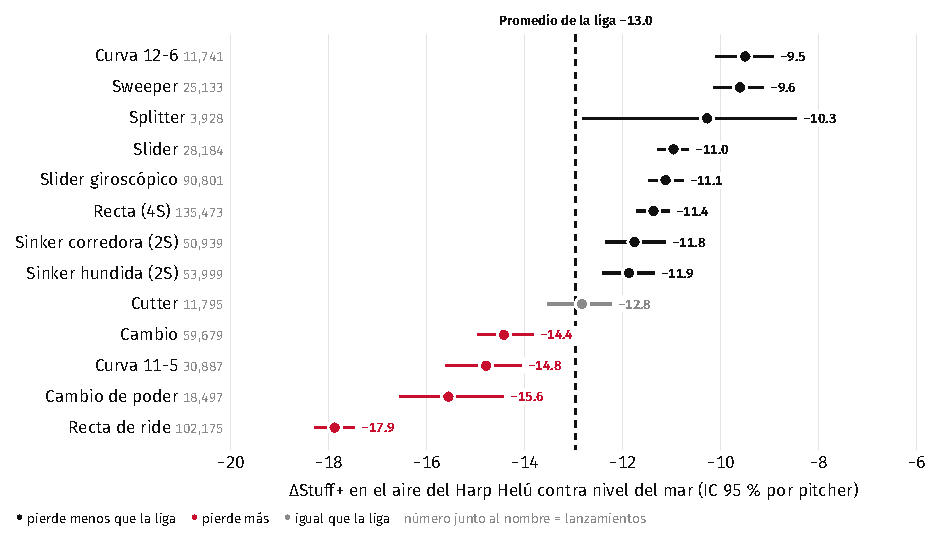
\includegraphics[width=0.92\linewidth,height=\textheight,keepaspectratio,alt={ΔStuff+
por forma de lanzamiento en el aire del Harp Helú, Stuff+
v2.}]{figures/forest_by_shape.pdf}
\caption{ΔStuff+ por forma de lanzamiento en el aire del Harp Helú,
Stuff+ v2.}
\end{figure}

\textbf{En términos absolutos todas las formas pierden.} La recta de
\emph{ride} pierde 5.3'' de subida y 2.7 pp de swings fallidos: su valor
depende de una subida que viene del giro. El HR/FB modelado sube en
todas las formas, de +1.0 pp (sweeper) a +6.2 pp (splitter)
(\texttt{reports/altitude\_delta/delta\_by\_shape.csv}).

\textbf{Triangulación con lo observado.} Comparamos el \emph{mismo}
lanzamiento (pitcher × temporada × \texttt{pitch\_id}) en juegos de
altitud extrema contra juegos sin altitud. El Stuff+ del modelo se mueve
en la misma dirección que el contrafactual en 7 de 7 familias; los
resultados reales del pitcher caen entre −7.5 y −15.3 puntos y su IC
contiene al contrafactual en 7 de 7
(\texttt{reports/altitude\_delta/triangulation.csv}).

\textbf{¿Física o aprendizaje? (HACK-084).} En una muestra de 20,000
lanzamientos, el ΔStuff+ de la liga en el aire del Harp Helú es −12.94.
Si solo se traslada el movimiento y el rasgo \texttt{rho} del modelo se
deja a nivel del mar, el lanzamiento pierde 5.95 puntos: es lo que quita
perder Magnus. Si el movimiento queda fijo y solo cambia el \texttt{rho}
aprendido, pierde 6.22: es lo que el modelo aprendió de los juegos en
altura, donde el contacto hace más daño y la bola vuela más. La
interacción suma los 0.77 restantes. Casi la mitad del efecto es física
medida y la otra mitad es el resultado aprendido
(\texttt{reports/model\_audit/decomposition.csv}).

\textbf{Parque por parque.} El Stuff+ neutral va de 98.1 a 102.0 en
todos los parques: los pitchers son comparables y lo que cambia es el
aire. El efecto del aire va de +4.7 en el parque más denso (\(\rho\) =
1.055) a −13.7 en el más ligero (\(\rho\) = 0.812)
(\texttt{reports/leaderboards/by\_park.csv}). En el staff candidato, el
ΔCDMX del modelo correlaciona 0.53 y 0.69 (por franquicia) con el delta
observado de cada pitcher (\texttt{reports/staff\_audit/README.md}).

\section{Recomendaciones y valor de
negocio}\label{recomendaciones-y-valor-de-negocio}

\textbf{De puntos a victorias (HACK-035).} Regresamos el valor de
carreras realizado contra los puntos de Stuff+ predichos fuera de
pliegue: un punto vale \(8.68\times10^{-4}\) carreras por lanzamiento
{[}\(8.18\times10^{-4}\), \(9.19\times10^{-4}\){]}. El exponente
pitagórico de la LMB es 1.90 {[}1.62, 2.15{]}: 11.8 carreras por
victoria en la liga y 14.3 en altitud extrema, donde se anota más. +10
puntos de Stuff+ en 2,500 lanzamientos son 21.7 carreras ≈ 1.51
victorias en el Harp Helú; una desviación estándar observada entre
pitcher-temporadas (5.08 puntos) vale 0.77 victorias. Los puntos son los
de Stuff+ v2 fuera de pliegue (\texttt{reports/business\_value/}).

\textbf{Perfil a reclutar (HACK-017, HACK-022).} Umbrales y formas salen
de Stuff+ v2 (HACK-017 regenerado en HACK-083).

\begin{enumerate}
\def\labelenumi{\arabic{enumi}.}
\tightlist
\item
  \textbf{No pagar por \emph{ride} de recta.} El rango de Stuff+ entre
  IVB bajo y alto es 21.1 puntos a nivel del mar y solo 5.8 en el Harp
  Helú (\texttt{reports/recommendations/memo.md}).
\item
  \textbf{Extensión alta.} El quintil superior (6.43 ft o más) pierde
  11.0 puntos y el inferior 15.3
  (\texttt{reports/recommendations/memo.md}).
\item
  \textbf{Ángulo de llegada plano, neto de la altura de salida.} El
  quintil más plano pierde 12.4 puntos y el más inclinado 14.1: la
  brecha es menor que la de la extensión, pero sus intervalos no se
  traslapan (\texttt{reports/recommendations/memo.md}).
\item
  \textbf{Secundarios.} Preferir curva 12-6, sweeper y splitter;
  desconfiar del cambio de poder y de la curva 11-5. Sin umbral de
  velocidad: su efecto no es robusto.
\end{enumerate}

La diferencia de pérdida entre la recta de \emph{ride} y el sweeper (8.3
puntos) equivale a unas 7.2 carreras por cada 1,000 lanzamientos
(\texttt{reports/recommendations/memo.md}).

\textbf{Staff candidato (HACK-032).} Para las dos franquicias
candidatas, siempre por separado porque la identificación es inferida:
22 de 35 y 25 de 45 pitchers tienen un lanzamiento 5 puntos o más peor
en aire del Harp Helú que su mejor lanzamiento. Moverle 10 puntos de uso
en casa ahorra 2.3 y 5.2 carreras por temporada, y pasar aperturas en
casa al abridor más resistente a la altura suma 2.18 y 1.38.
\textbf{Total: 4.5 y 6.5 carreras por temporada (0.32 y 0.46 victorias)}
con los juegos en casa observados
(\texttt{reports/staff\_audit/README.md}).

\textbf{Tácticas en casa (hipótesis del modelo de ubicación).} El centro
de la zona es lo que más se encarece en el aire del Harp Helú (recta en
la zona 4: +0.027 carreras por lanzamiento) y la esquina baja del lado
del guante la que mejor aguanta (+0.006)
(\texttt{reports/location\_model/altitude\_by\_zone.csv}).

Todo esto se consulta en el producto web: simulador 3D CDMX contra nivel
del mar con el motor de vuelo medido, explicador de física,
leaderboards, altitud, staff, prospectos, laboratorio de diseño y
metodología.

\section{Alcance y fronteras}\label{alcance-y-fronteras}

\begin{itemize}
\tightlist
\item
  \textbf{Fuera de alcance:} seguimiento de corredores (no está en los
  datos) y datos externos de MLB para entrenar.
\item
  \textbf{Limitaciones, cada una con su evidencia:}

  \begin{enumerate}
  \def\labelenumi{\arabic{enumi}.}
  \tightlist
  \item
    \textbf{CDMX frente a Puebla} no se distinguen
    (\(P = 0.832 < 0.95\), §3): \(\hat\rho_{HH}\) usa las dos
    franquicias juntas y el staff se reporta por separado
    (\texttt{reports/park\_id/harp\_helu.md}).
  \item
    \textbf{Residuo de sustentación sin explicar} (§4.1): por eso la
    traducción usa la elasticidad medida y no la eficiencia de giro.
  \item
    \textbf{Preparación transductiva.} Identidad, densidad por juego,
    referencias de arsenal y valores de carrera se estiman una vez con
    todos los datos; ningún paso usa el resultado de un lanzamiento como
    variable de ese lanzamiento y todos los modelos se ajustan solo con
    entrenamiento.
  \item
    \textbf{\(\rho\) es por juego} y puede absorber rasgos del parque
    que viajan con la altitud; la triangulación dentro del lanzamiento y
    el holdout por parque acotan ese riesgo.
  \item
    \textbf{R3 no se cumplió.} Stuff+ v2 cambia la magnitud del efecto
    de la altitud (§5); se adoptó por la regla del sesgo en aire no
    visto, y el orden de las formas se conserva.
  \item
    \textbf{La conversión a carreras es lineal} en los puntos de Stuff+
    y usa las carreras por victoria de un equipo promedio: es un orden
    de magnitud, no una promesa (§7).
  \item
    \textbf{Incertidumbre individual grande.} El intervalo del ΔStuff+
    observado de un pitcher mide ±7.6 puntos (§5.1): el modelo da la
    expectativa, no el caso (\texttt{reports/uncertainty/README.md}).
  \item
    \textbf{Las recomendaciones tácticas y de mezcla son hipótesis del
    modelo}, no experimentos.
  \item
    \textbf{Traductor del cutter y del splitter.} La traducción
    proporcional se dispara cuando el movimiento medio está cerca de 0.
    Para el HB del cutter predice +9.29 in contra +1.44 in observados
    (cociente 6.45, 1.9 \% de los lanzamientos), y para el del splitter
    +1.31 contra +1.85 (cociente 0.71, 0.6 \%). Las familias calibradas
    en sus dos componentes suman 97.5 \% de los lanzamientos; el ΔStuff+
    de esas dos familias se lee con cautela
    (\texttt{reports/model\_audit/calibration.csv},
    \texttt{reports/model\_audit/README.md}).
  \end{enumerate}
\item
  \textbf{Ética:} IDs anónimos, sin fines de apuesta, y los datos crudos
  nunca están en git ni en el despliegue (solo agregados).
\end{itemize}

\section*{Referencias}\label{referencias}
\addcontentsline{toc}{section}{Referencias}

\protect\phantomsection\label{refs}
\begin{CSLReferences}{1}{0}
\bibitem[\citeproctext]{ref-angelopoulos2021gentle}
Angelopoulos, Anastasios N., y Stephen Bates. 2021. \emph{A Gentle
Introduction to Conformal Prediction and Distribution-Free Uncertainty
Quantification}. \url{https://arxiv.org/abs/2107.07511}.

\bibitem[\citeproctext]{ref-driveline2021stuff}
Baseball, Driveline. 2021. \emph{What is Stuff+? Quantifying Pitches
with Pitch Models}. Driveline Baseball (blog); actualización de método
en 2024: Revisiting Stuff+.
\url{https://drivelinebaseball.com/blogs/blog/what-is-stuff-quantifying-pitches-with-pitch-models}.

\bibitem[\citeproctext]{ref-blondel2008louvain}
Blondel, Vincent D., Jean-Loup Guillaume, Renaud Lambiotte, y Etienne
Lefebvre. 2008. {«Fast unfolding of communities in large networks»}.
\emph{Journal of Statistical Mechanics: Theory and Experiment}, P10008.
\url{https://arxiv.org/abs/0803.0476}.

\bibitem[\citeproctext]{ref-grove_pitchingbot}
Grove, Cameron. s.~f. \emph{PitchingBot Pitch Modeling Primer}.
FanGraphs Sabermetrics Library.
\url{https://library.fangraphs.com/pitching/pitchingbot-pitch-modeling-primer}.

\bibitem[\citeproctext]{ref-guo2017calibration}
Guo, Chuan, Geoff Pleiss, Yu Sun, y Kilian Q. Weinberger. 2017. {«On
Calibration of Modern Neural Networks»}. \emph{Proceedings of the 34th
International Conference on Machine Learning (PMLR 70)}, 1321-30.
\url{https://proceedings.mlr.press/v70/guo17a.html}.

\bibitem[\citeproctext]{ref-kagan2014drag}
Kagan, David, y Alan M. Nathan. 2014. {«Simplified Models for the Drag
Coefficient of a Pitched Baseball»}. \emph{The Physics Teacher}, 52,
278.
\url{https://physics.csuchico.edu/kagan/professional/papers/drag.pdf}.

\bibitem[\citeproctext]{ref-ke2017lightgbm}
Ke, Guolin, Qi Meng, Thomas Finley, et~al. 2017. {«LightGBM: A Highly
Efficient Gradient Boosting Decision Tree»}. \emph{Advances in Neural
Information Processing Systems 30 (NIPS 2017)}.
\url{https://papers.nips.cc/paper/2017/hash/6449f44a102fde848669bdd9eb6b76fa-Abstract.html}.

\bibitem[\citeproctext]{ref-fangraphs_lw}
\emph{Linear Weights}. s.~f. FanGraphs Sabermetrics Library.
\url{https://library.fangraphs.com/principles/linear-weights}.

\bibitem[\citeproctext]{ref-lundberg2017shap}
Lundberg, Scott M., y Su-In Lee. 2017. {«A Unified Approach to
Interpreting Model Predictions»}. \emph{Advances in Neural Information
Processing Systems 30 (NIPS 2017)}.
\url{https://arxiv.org/abs/1705.07874}.

\bibitem[\citeproctext]{ref-mcgrattan2023primer}
McGrattan, Owen. 2023. \emph{Stuff+, Location+, and Pitching+ Primer}.
FanGraphs Sabermetrics Library.
\url{https://library.fangraphs.com/pitching/stuff-location-and-pitching-primer}.

\bibitem[\citeproctext]{ref-nathan2021hawkeye}
Nathan, Alan M. 2021. \emph{Hawkeye Spin Analysis, Part I: Determining
Magnus and non-Magnus Movement}.
\url{https://baseball.physics.illinois.edu/HawkeyeSpinAnalysis-Part\%20I-rev1.pdf}.

\bibitem[\citeproctext]{ref-nathan2006spin}
Nathan, Alan M., Joe Hopkins, Lance Chong, y Hank Kaczmarski. 2006.
\emph{The Effect of Spin on the Flight of a Baseball}.
\url{https://arxiv.org/abs/physics/0605041}.

\bibitem[\citeproctext]{ref-richardson2014altitude}
Richardson, Eliza. 2014. {«High Altitude Offense: An Empirical
Examination of the Relationship Between Runs Scored and Stadium
Elevation»}. \emph{Baseball Research Journal (SABR)}.
\url{https://sabr.org/journal/article/high-altitude-offense-an-empirical-examination-of-the-relationship-between-runs-scored-and-stadium-elevation/}.

\bibitem[\citeproctext]{ref-shimodaira2000covariate}
Shimodaira, Hidetoshi. 2000. {«Improving predictive inference under
covariate shift by weighting the log-likelihood function»}.
\emph{Journal of Statistical Planning and Inference}, 90, 227-44.

\bibitem[\citeproctext]{ref-suttonbrown2024stuffpro}
Sutton-Brown, Stephen. 2024. \emph{Introducing StuffPro and PitchPro}.
Baseball Prospectus.
\url{https://www.baseballprospectus.com/news/article/89245/stuffpro-pitchpro-introduction-new-pitch-metrics-bp/}.

\bibitem[\citeproctext]{ref-tango2008woba}
Tango, Tom. 2008. \emph{The Joy of wOBA}. FanGraphs Blog.
\url{https://blogs.fangraphs.com/the-joy-of-woba/}.

\bibitem[\citeproctext]{ref-tibshirani2019conformal}
Tibshirani, Ryan J., Rina Foygel Barber, Emmanuel J. Candès, y Aaditya
Ramdas. 2019. {«Conformal Prediction Under Covariate Shift»}.
\emph{Advances in Neural Information Processing Systems 32 (NeurIPS
2019)}. \url{https://arxiv.org/abs/1904.06019}.

\end{CSLReferences}

\end{document}
